
\documentclass{include/thesisclass3}

\SelectLanguage{ngerman}
\usepackage{float}
      

% Titlepage settings
\newcommand{\praktikum}{Praktikum moderne Physik}
\newcommand{\autora}{Jens Schäfer}
\newcommand{\autorb}{Jan van der Linden}
\newcommand{\maila}{ugecd@student.kit.edu}
\newcommand{\mailb}{jan.vdlinden95@gmail.com}
\newcommand{\topic}{Quantenradierer}
\newcommand{\ptime}{22. Mai 2017}


% Shortcuts
\newcommand{\cc}{\cdot}
\newcommand{\rk}{\rangle}
\newcommand{\lk}{\langle}
\newcommand{\df}{\rightarrow}
\newcommand{\la}{\lambda}
\newcommand{\dd}{{\rm d}}
\newcommand{\ehm}{\mathbbm{1}}
\newcommand{\p}{\partial}
\newcommand{\soll}{\overset{!}{=}}
\newcommand{\D}{\Delta}
\newcommand{\eps}{\epsilon}
\newcommand{\vektor}[3]{\begin{pmatrix} #1 \\ #2 \\ #3 \end{pmatrix}}
\newcommand{\vektorz}[2]{\begin{pmatrix} #1 \\ #2 \end{pmatrix}}
\newcommand{\Mat}[9]{\begin{pmatrix}#1&#2&#3\\#4&#5&#6\\#7&#8&#9\end{pmatrix}}
\newcommand{\Matz}[4]{\begin{pmatrix}#1&#2\\#3&#4\end{pmatrix}}
\newcommand{\e}[1]{\,\si{#1}}
 


\begin{document}

	\FrontMatter
	% coordinates for background border
\newcommand{\diameter}{20}
\newcommand{\xone}{-15}
\newcommand{\xtwo}{160}
\newcommand{\yone}{15}
\newcommand{\ytwo}{-253}




\begin{titlepage}
    % background border
    \begin{tikzpicture}[overlay]
    \draw[color=gray]
            (\xone mm, \yone mm)
      -- (\xtwo mm, \yone mm)
    arc (90:0:\diameter pt)
      -- (\xtwo mm + \diameter pt , \ytwo mm)
        -- (\xone mm + \diameter pt , \ytwo mm)
    arc (270:180:\diameter pt)
        -- (\xone mm, \yone mm);
    \end{tikzpicture}



    % KIT image and sign for faculty of physics
    \begin{textblock}{10}[0,0](4.5,2.5)
        
\includegraphics[width=.25\textwidth]{include/kitlogo.pdf}
    \end{textblock}
    

    % horizontal line
    \begin{textblock}{10}[0,0](4.2,3.1)
        \begin{tikzpicture}[overlay]
        \draw[color=gray]
                (\xone mm + 5 mm, -12 mm)
          -- (\xtwo mm + \diameter pt - 5 mm, -12 mm);
        \end{tikzpicture}
    \end{textblock}



    % begin of text part
    \changefont{phv}{m}{n}    % helvetica
    \centering



    % thesis topic (en and ge)
    \vspace*{3cm}
    \Huge\praktikum\\



    % author name and institute
    \vspace*{5cm}
    
    \huge\topic\\






    % examiners (Referenten)
    \vspace*{3cm}
    \Large
    \begin{center}
        \begin{tabular}[ht]{l c l } 
  \autora & \hfill & \textit{\maila} \\
\autorb & \hfill & \textit{\mailb} \\
        
        \end{tabular}
    \end{center}



    % working time
    \vspace{2cm}
    \begin{center}
        \large{Durchgeführt am}: \ptime
    \end{center}



    % lowest text blocks concerning the KIT
    \begin{textblock}{10}[0,0](4,16.8)
        \tiny{KIT -- Universität des Landes Baden-Württemberg und nationales %
              Forschungszentrum in der Helmholtz-Gemeinschaft}
    \end{textblock}
    \begin{textblock}{10}[0,0](14,16.75)
        \large{\textbf{www.kit.edu}}
    \end{textblock}
\end{titlepage}

	\tableofcontents                  
	\newpage
	\MainMatter

%Protokollstart

\chapter{Theoretische Grundlagen}

\section{Ziel des Experiments}

In diesem Experiment werden quantenmechanische Eigenschaften wie die Aufenthaltswarscheinlichkeit von Teilchen anschaulich dargestellt. Hierzu werden kohärente Photonen zur Interferenz im Mach-Zehnder-Interferometer gebracht. 

\section{Durchführung}
\begin{figure}[H]
	\begin{center}
		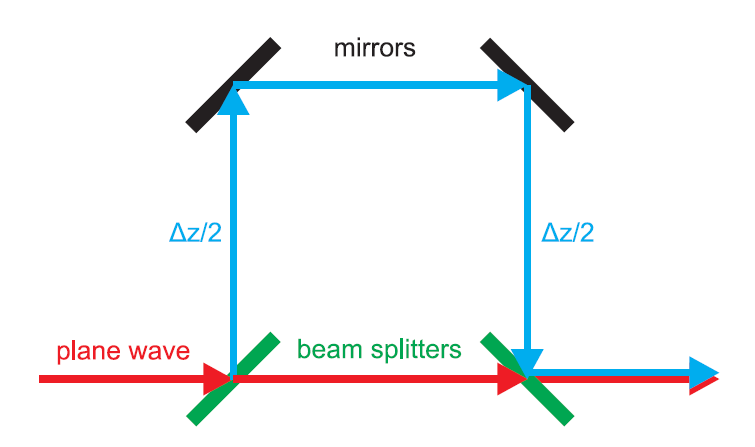
\includegraphics[width=0.8\textwidth]{images/Beamsplit.png}
		\caption{Mach-Zender-Interferometer, Quelle: Quantum Eraser, KSOP Optics \& Photonics Lab}
		\label{Mach-Zehnder}
	\end{center}
\end{figure}

In Abbildung \ref{Mach-Zehnder} ist ein Mach-Zehnder-Interferometer dargestellt. Ein Lichtstrahl wird dabei durch einen ersten Beamsplitter aufgeteilt. Der erste Strahl verläuft geradlinig weiter, der Zweite wird durch zwei Spiegel auf einen um $\Delta z/2$ längeren Umweg geführt. Nach dem Umweg werden die Teilstrahlen durch einen zweiten Beamsplitter wieder zusammengeführt, sodass sie fortan in einer Bahn weiter laufen. Als Lichtquelle wird ein Laser verwendet, somit sind die Teilstrahlen kohärent und gut fokusiert. Nach dem zweiten Beamsplitter bilden sich zwei Richtungen für die rekombinierten Strahlen aus, beide werden auf seperaten Schirmen abgebildet, wie in Abb. \ref{Aufbau} ersichtlich. 
\begin{figure}[H]
	\begin{center}
		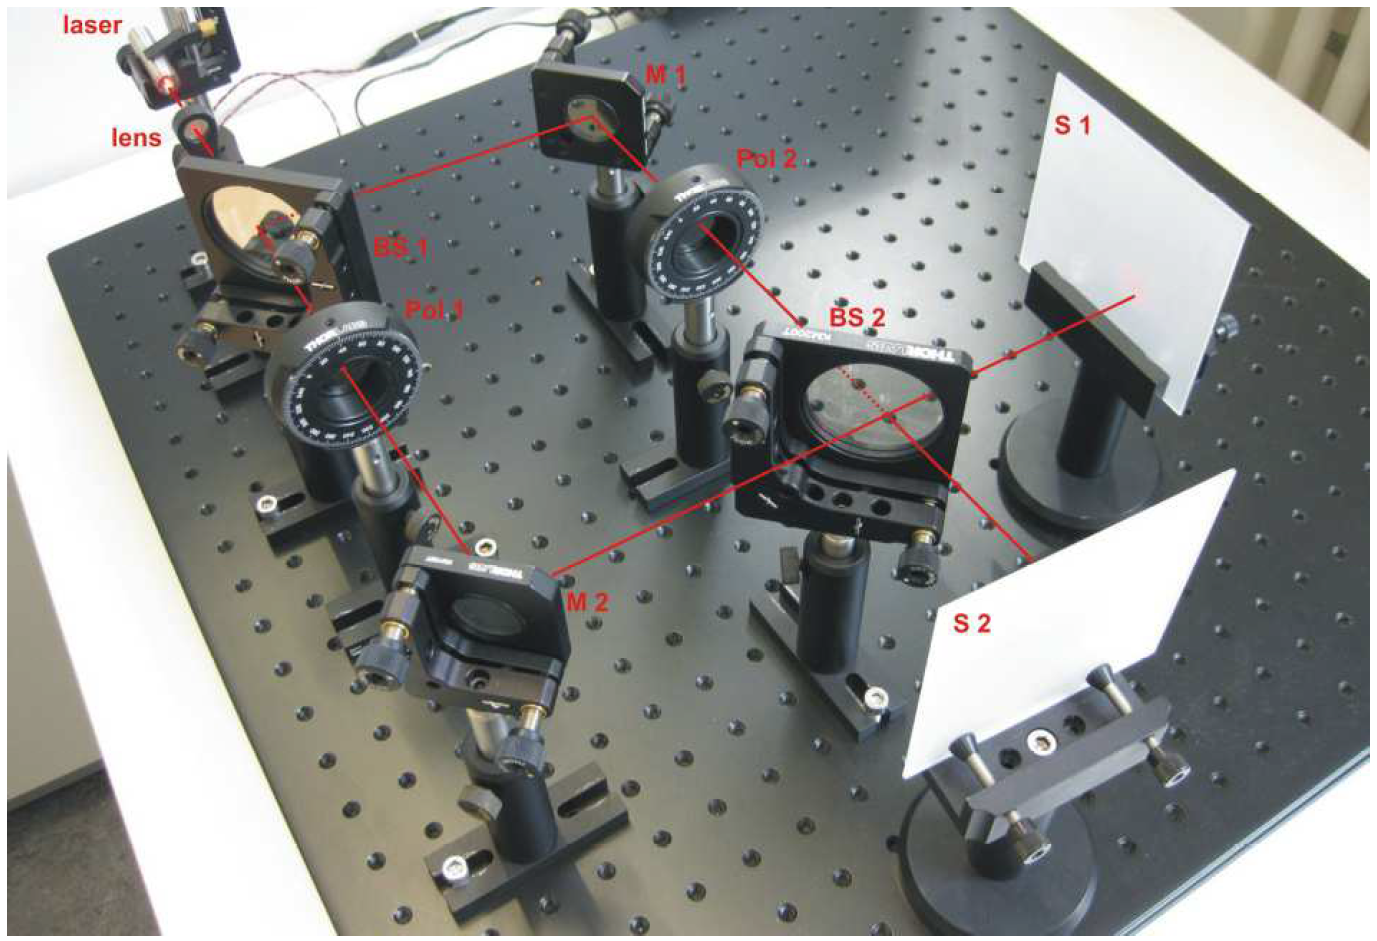
\includegraphics[width=0.8\textwidth]{images/Aufbau.png}
		\caption{Experimenteller Aufbau, Quelle: Quantum Eraser, KSOP Optics \& Photonics Lab}
		\label{Aufbau}
	\end{center}
\end{figure}
\subsection{Wellendynamik}
Die Photonendichte ist proportional zur Lichtintensität und gegeben mit:
\begin{equation}
n_{ph}(z,t)=\frac{I(\vec{x},t)}{\hbar \omega}=\frac{\vert \vec{E}\vert ^2}{\hbar \omega}
\end{equation}
Geht man von idealen Bedingungen aus, sollte sich klassisch gesehen die Teilchendichte nach Aufteilen und wieder Zusammenführen eines Strahls nicht verändern. Bei dem Interferometer gibt es einen Phasenunterschied zwischen den Teilstrahlen, welcher durch den Gangunterschied $\Delta z$ parametrisiert ist. Hinter dem zweiten Beamsplitter werden die zwei Strahlen wieder vereint, wobei $\vec{E_0}$ die Feldstärke der Quelle ist:
\begin{align}
\si{Strahl\, A}\quad \vec{E}_A(z,t)&=\frac{1}{4}\vec{E_0}e^{i(k_z z-\omega t)}\\
\si{Strahl\, B}\quad \vec{E}_B(z,t)&=\frac{1}{4}\vec{E_0}e^{i(k_z (z+\Delta z)-\omega t)}
\end{align}
Hierbei ist die Feldstärke eines jeden Teilstrahls auf ein Viertel abgesunken, da sie bei zwei Beamsplittern jeweils halbiert wurde. Die Superposition der zusammengeführten Teilstrahlen ergibt sich somit zu:
\begin{equation}
\vec{E}_{ges}(z,t)= \vec{E}_A+\vec{E}_B=\frac{1}{4}\vec{E_0}(e^{ik_z z}+e^{ik_z (z+\Delta z)})e^{i\omega t}
\end{equation}
Daraus ergibt sich die Photonendichte für einen der beiden rekombinierten Strahlen hinter dem zweiten Beamsplitter zu:
\begin{equation}
n_{ph}(z,t)=\frac{\vert \vec{E}_{ges} \vert ^2}{\hbar \omega}=\frac{\vert \vec{E}_0\vert ^2}{4\hbar\omega}(1+\cos(k_z\Delta z))\label{n}
\end{equation}
Klassisch ist der Interferenzterm $(1+\cos(k_z z))$ nicht erklärbar, das Ergebnis der Photonendichte wäre $\frac{\vert \vec{E}_0\vert}{2\hbar \omega}$ also gerade die Hälfte der Quelle und das Maximum von \ref{n}, da nach dem zweiten Beamsplitter der Grundstrahl effektiv halbiert wurde. 
\section{Quantenradierer}
Im Experiment wird nun das Mach-Zehnder-Interferomenter wie in Abb. \ref{Aufbau} dargestellt, mit einen Polarisationsfilter pro Strahlgang ausgebaut. Geht man von einer, in X-Richtung polarisierten Quelle aus und polarisiert die Strahlen in $\pm 45^\circ$ betragen die Felder der Teilstrahlen hinter dem zweiten Beamsplitter:
\begin{align}
\vec{E}_A&=\frac{E_0}{4}e^{i(k_z z - \omega t)} \cdot\frac{1}{\sqrt{2}}\left(\begin{array}{c} 1 \\ 1 \end{array}\right)\\
\vec{E}_B&=\frac{E_0}{4}e^{i(k_z (z+\Delta z) - \omega t)}\cdot \frac{1}{\sqrt{2}}\left(\begin{array}{c} 1 \\ -1 \end{array}\right)
\end{align}
Berechnet man nun für den rekombinierten Strahl die Photonendichte nach \ref{n}, so verschwindet durch die Orthogonalität der Teilstrahlen der Interferenzterm. Damit fällt die Teilchendichte auf die Hälfte. Da der Interferenzterm verantwortlich für das Erscheinen des Interferenzmusters ist, sollte mit den Polfiltern auf keinem der beiden Schirmen Interferenz festgestellt werden können.\\
Nun wird vor einen der Schirme ein zusätzlicher Polarisator, der Quantenradierer positioniert. Dieser Polarisator wird mit $0^\circ$ respektive zur Polarisation der Quelle eingestellt und hat somit eine relative Polarisation von $\pm 45^{\circ}$ zu den einfallenden Teilstrahlen. Hierdurch werden die Teilstrahlen auf diese Polarisation projiziert, was mathematisch einer Drehung des Polarisationsvektors um $\pm 45^{\circ}$ entspricht. Dazu wird der Vektor des elektrischen Feldes wieder mit der Drehmatrix für 2D-Drehungen multipliziert. Die Wellen haben hinter dem Quantenradierer dann folgende Gestallt:
\begin{align}
\vec{E}_A&=\frac{E_0}{8}e^{i(k_z z - \omega t)} \cdot\left(\begin{array}{c} 1 \\ 0 \end{array}\right)\\
\vec{E}_B&=\frac{E_0}{8}e^{i(k_z (z+\Delta z) - \omega t)}\cdot \left(\begin{array}{c} 1 \\ 0 \end{array}\right)
\end{align}
Diese lineare Ausrichtung kann nun miteinander interferieren und für die Photonendichte ergibt sich:
\begin{equation}
n_{ph}(z,t)=\frac{\vert \vec{E}_0\vert ^2}{8\hbar\omega}(1+\cos(k_z\Delta z))
\end{equation}
Somit kann wieder ein Interferenzbild wahrgenommen werden.

\chapter{Durchführung}
\section{Justierung}
Zu Beginn des Experiments wurde das Interferometer aufgebaut (Abbildung \ref{aufbau}) und mit einem fokussierten Laser so justiert, dass die Strahlengänge beider Teilstrahlen hinter dem zweiten Strahlteiler wieder zusammenfallen. Durch eine Aufweitung des Ursprungsstrahls und weitere Feinjustierung konnte dann auf den Schirmen das gewünschte Interferenzmuster sichtbar gemacht werden (Abbildung \ref{interferenz}). Quantenmechanisch entspricht dies dem Verlust der Information, auf welchem Weg ein Photon zum Schirm gelangt, weshalb die Wahrscheinlichkeitsamplituden der Teilstrahlen miteinander interferieren.
\begin{figure}[H]
\centering
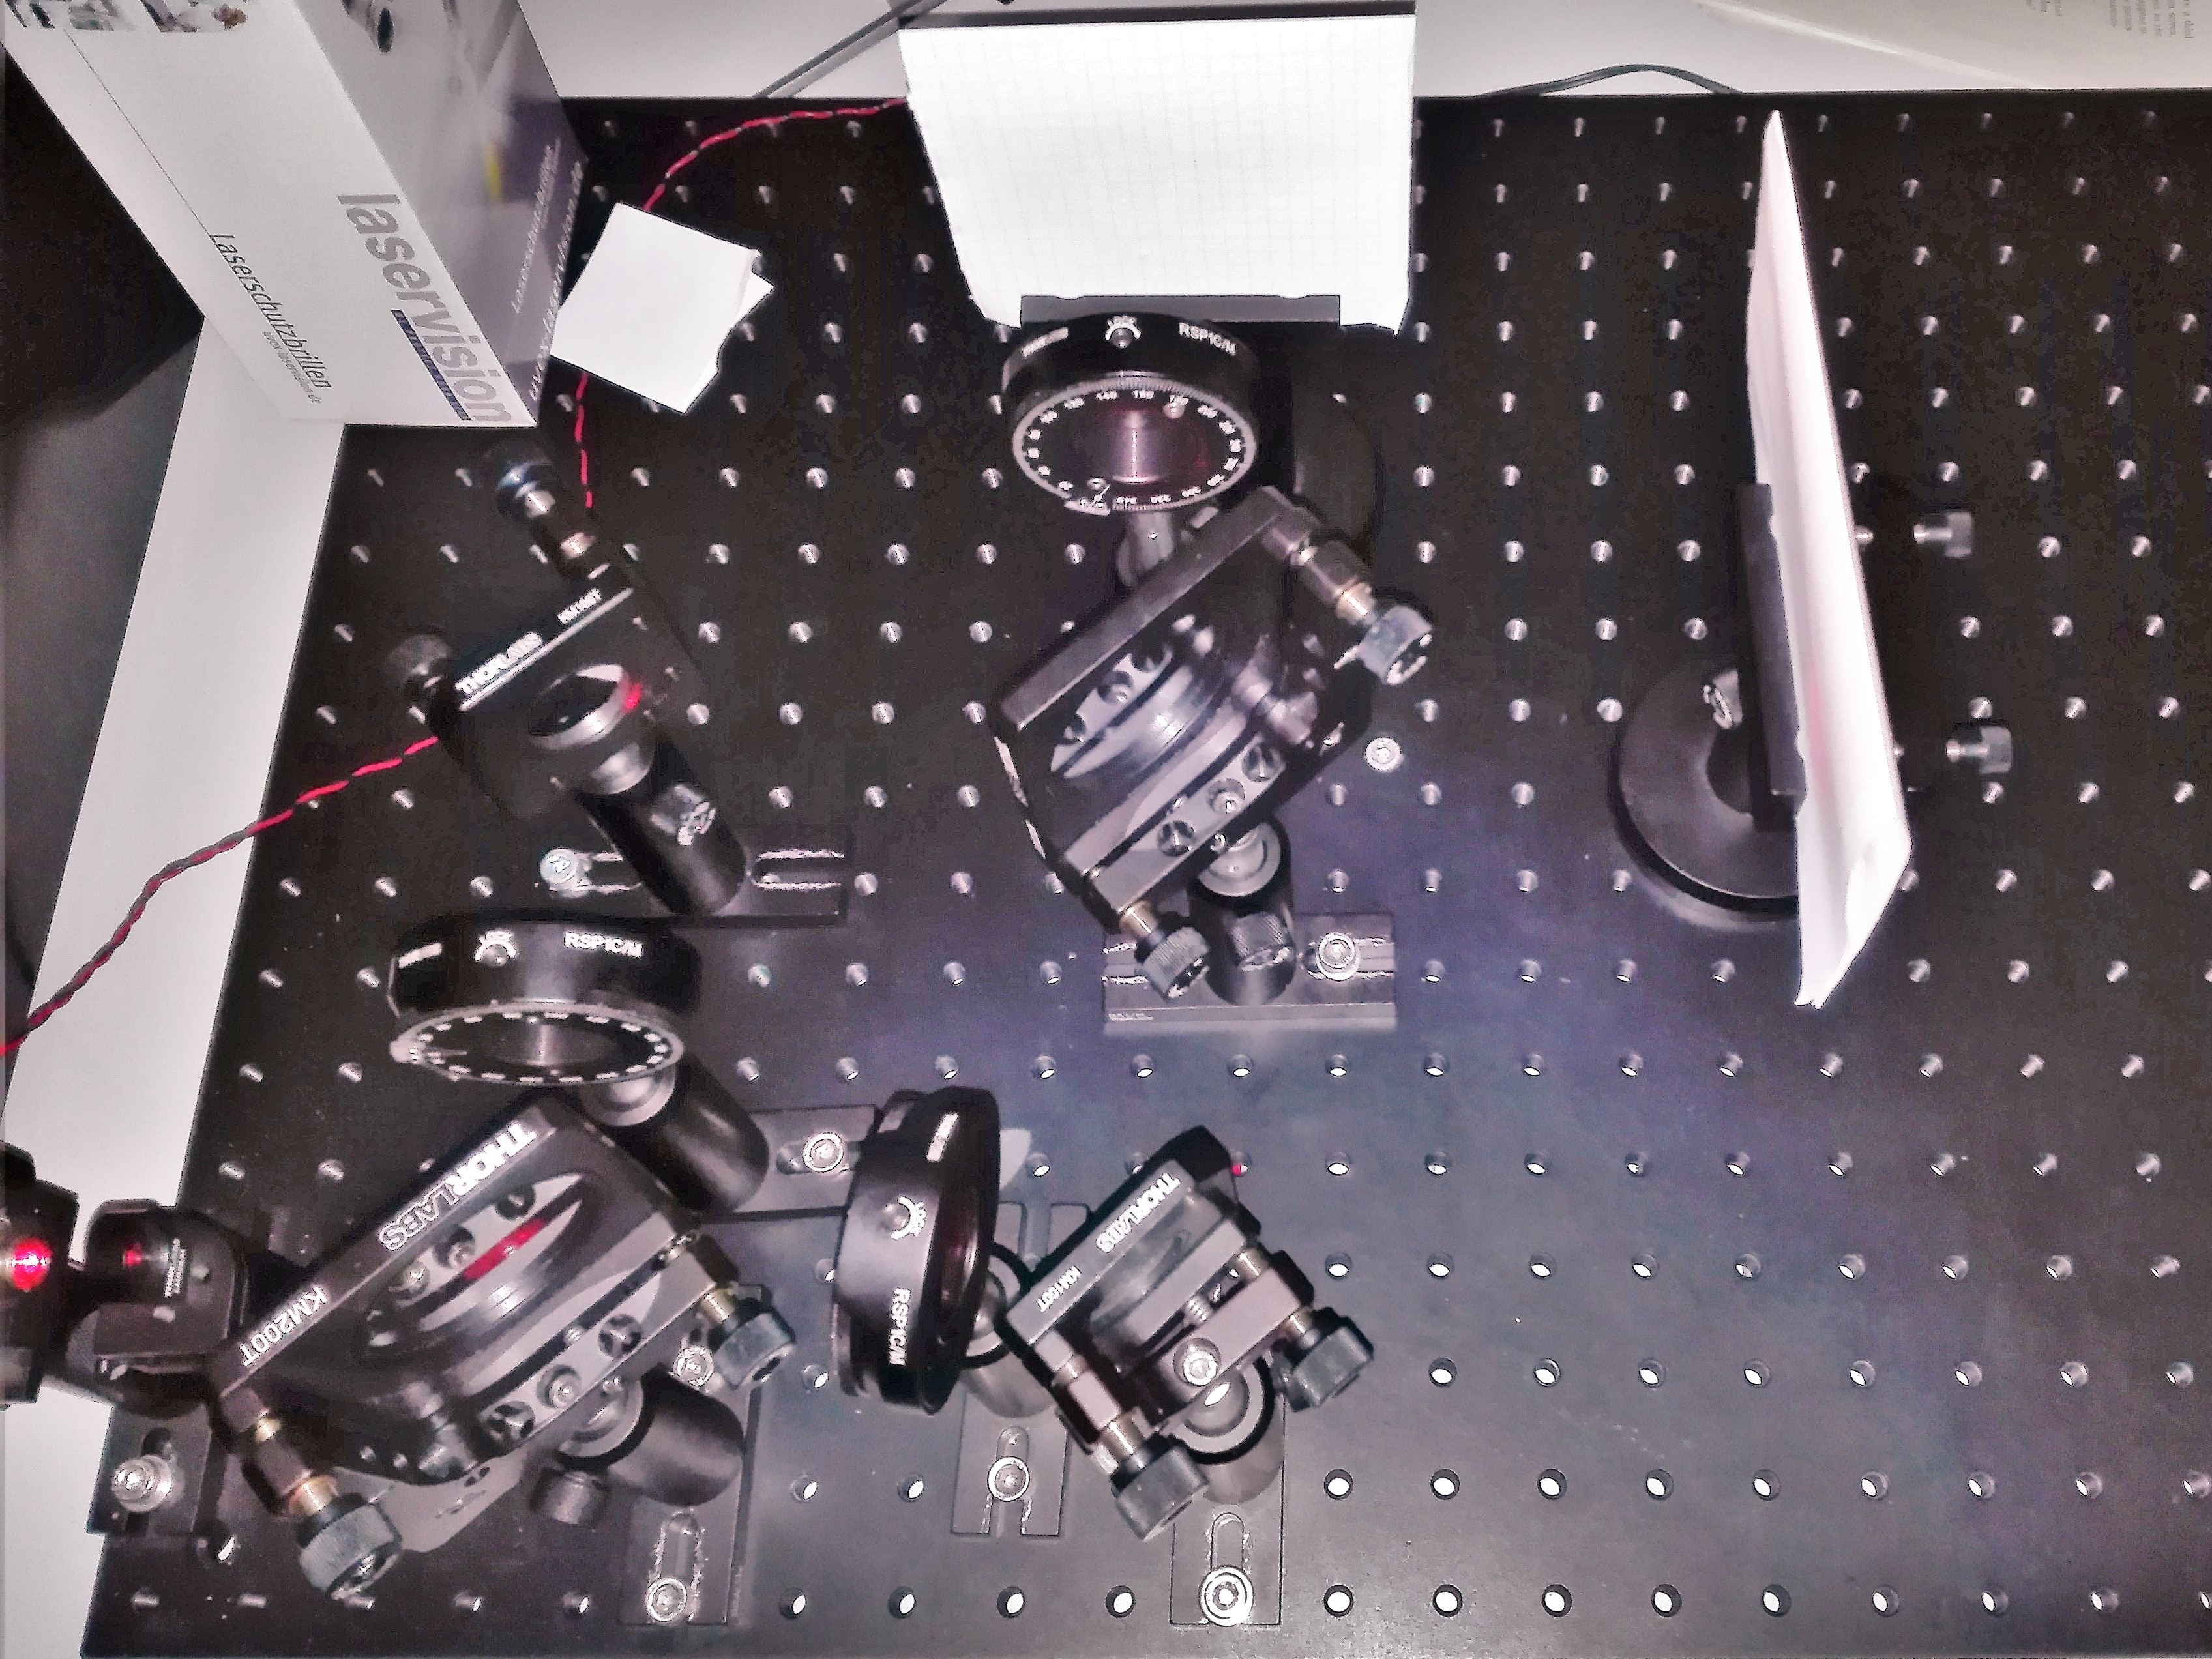
\includegraphics[scale=0.1]{images/eigener-aufbau.jpg}
\caption{Verwendeter Aufbau des Interferometers. Der Laser befindet sich in der unteren linken Ecke, direkt davor befindet sich eine Linse zur Aufweitung des Strahls. Der Strahlrichtung folgend, befindet sich dahinter ein Strahlteiler, welcher den Ursprungsstrahl gerade durch lässt und nach oben ablenkt. Im Stahlengang der beiden Teilstrahlen befinden sich jeh ein Polarisator mit relativen Polarisationswinkeln von $90^\circ$ zueinander. Die beiden Teilstrahlen werden beim Strahlteiler in der Mitte wieder vereint und auf die beiden weißen Schirme projiziert. Ebenso zu Sehen ist ein weiterer Polarisationsfilter unter dem oberen Schirm, der Quantenradierer. Dieser hat zu den beiden vorherigen Polarisatoren eine relative Ausrichtung von je $45^\circ$.}
\label{aufbau}
\end{figure}

\begin{figure}[H]
\centering
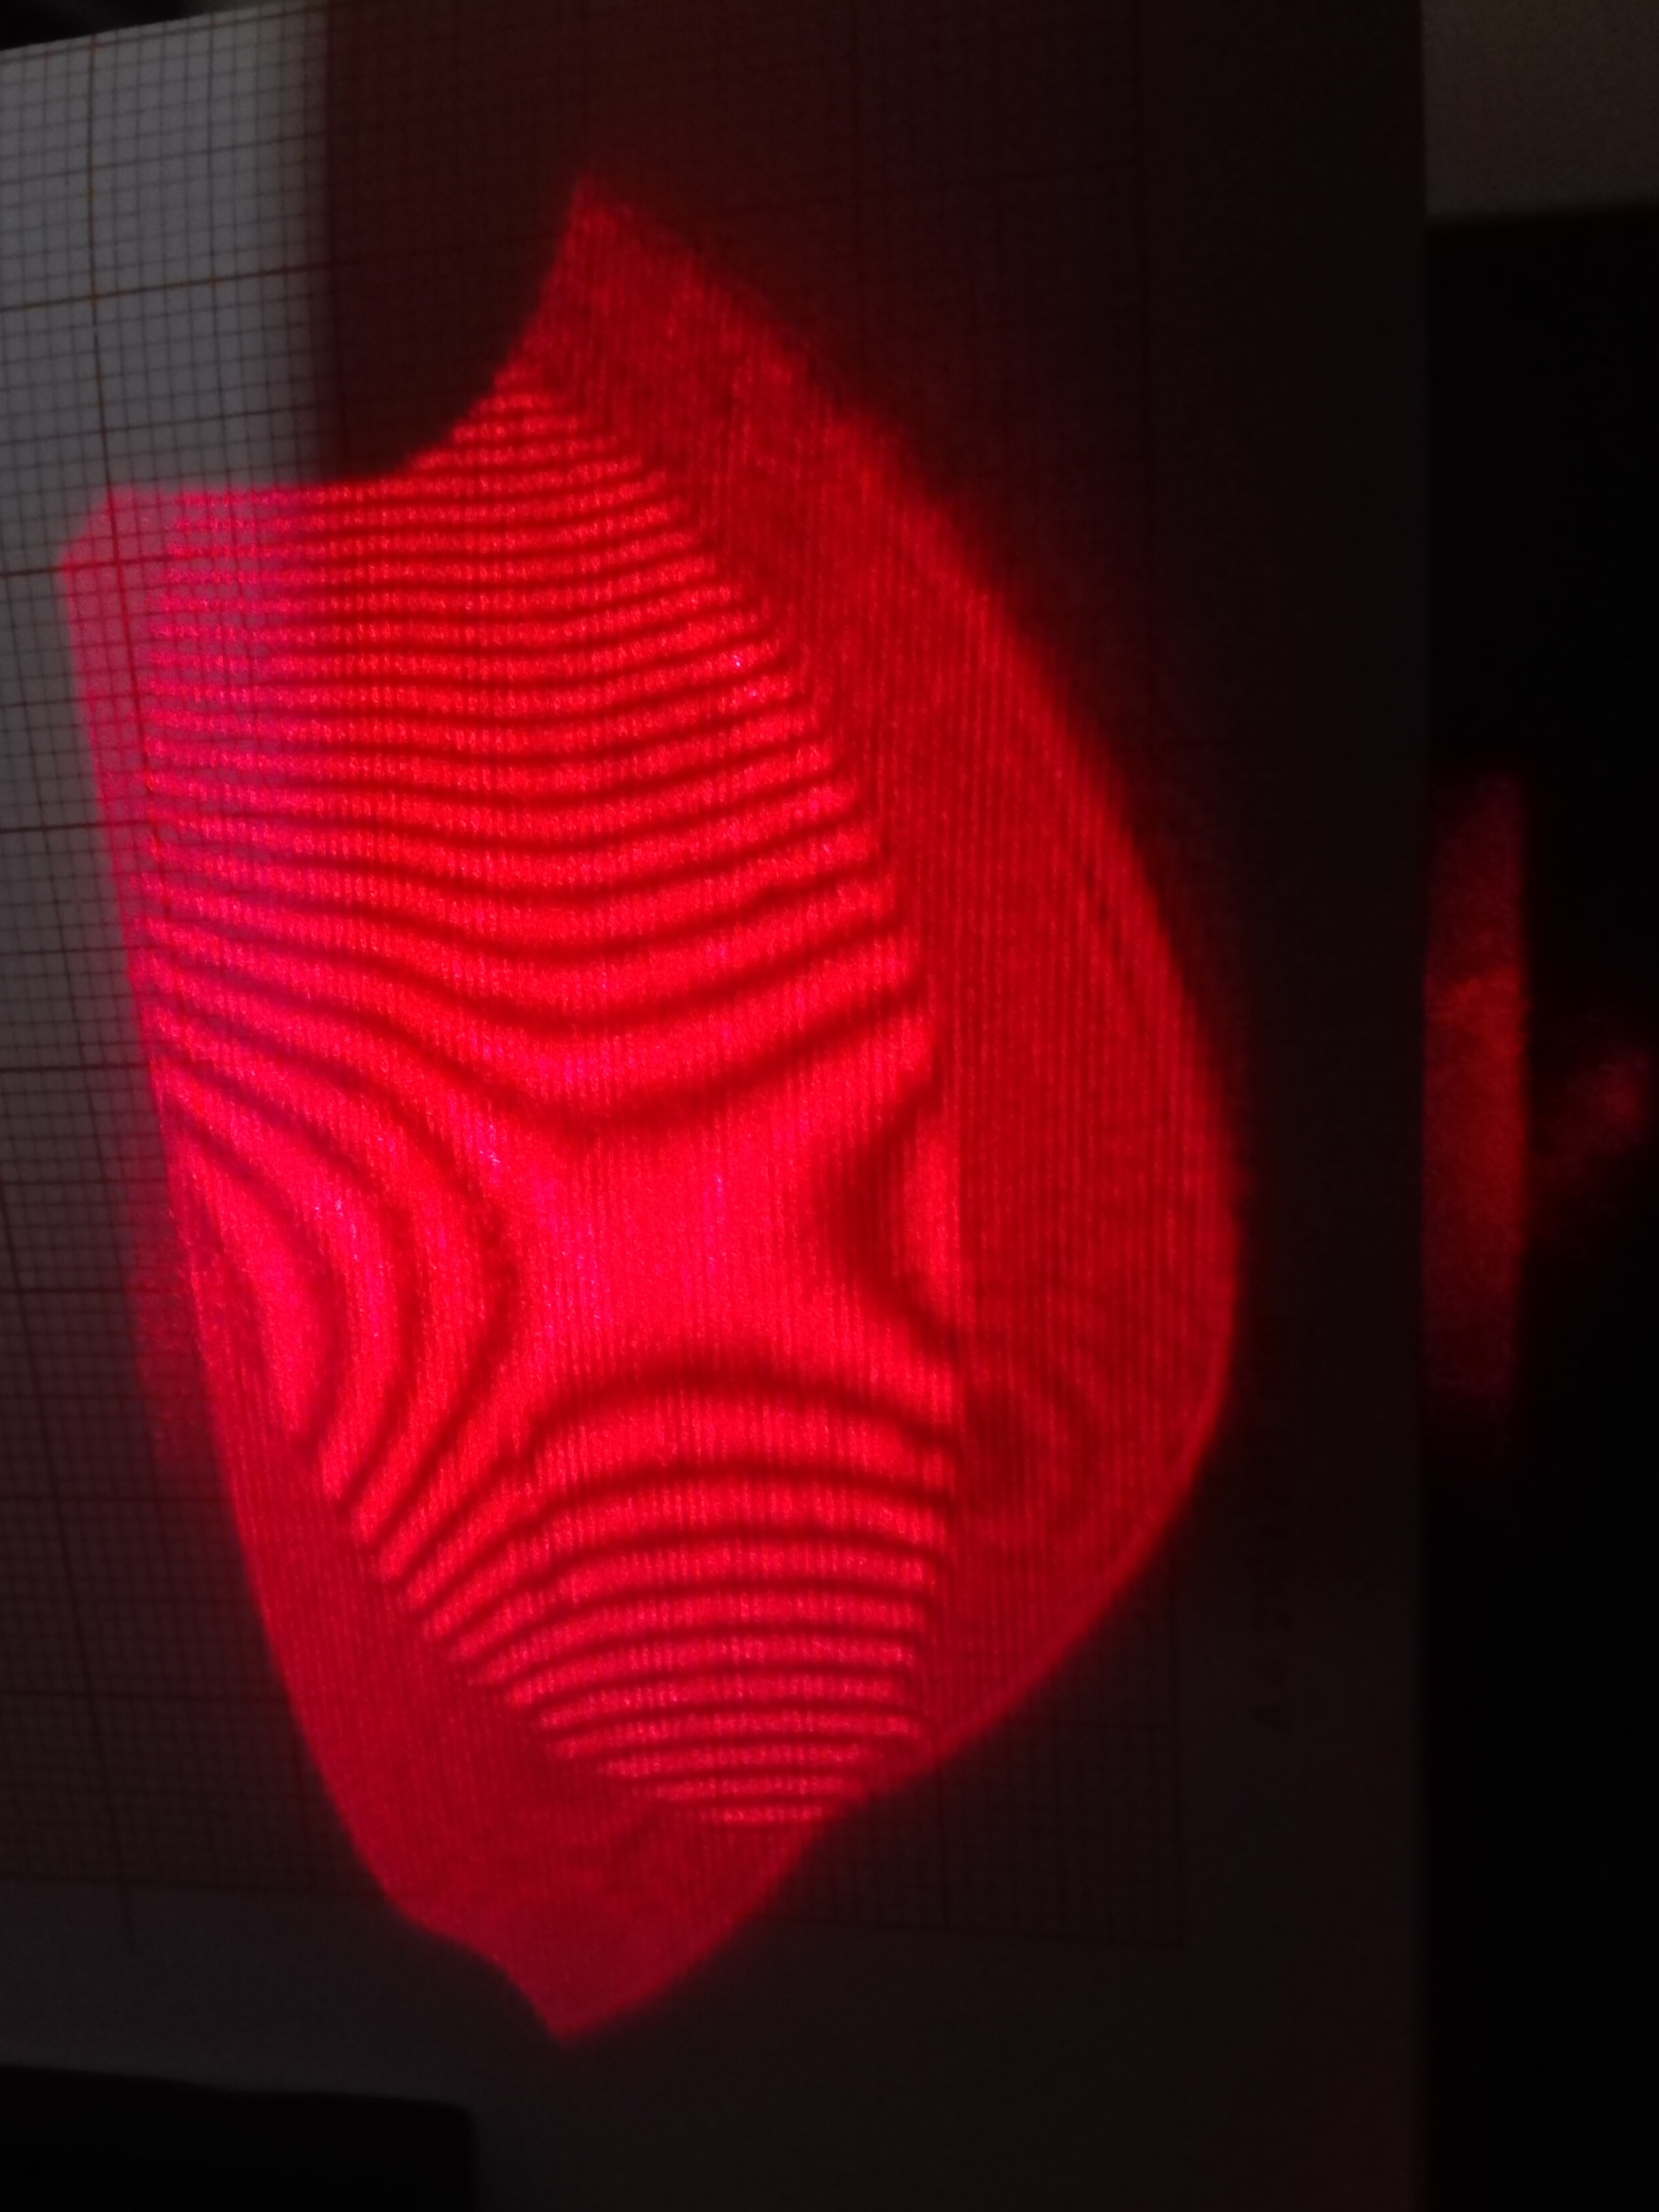
\includegraphics[scale=0.1]{images/interferenz.jpg}
\caption{Interferenzmuster des aufgeweiteten Laserstrahls an einem der Schirme. Durch den kontinuierlichen Gangunterschied der beiden Teilstrahlen entsteht im Idealfall ein Ringmuster.}
\label{interferenz}
\end{figure}
\section{Auflösen der Interferenz}
Durch die Positionierung je eines Polarisators in die beiden Teilstrahlen mit relativen Polarisationswinkeln von $90^\circ$ (auch Abbildung \ref{aufbau}) konnte das Interferenzmuster erfolgreich aufgelöst werden. Quantenmechanisch existiert durch die Polarisatoren eine Weginformation, es kann eine Aussage getroffen werden, auf welchem der beiden Wege ein Photon den Schrim erreicht.

\section{Der Quantenradierer}
Durch die Positionierung eines weiteren Polarisationsfilters  mit einer Ausrichtung von $45^\circ$ relativ zu den beiden anderen Polarisatoren (auch Abbildung \ref{aufbau}) vor einen der beiden Schirme konnte erneut ein Interferenzmuster beobachtet werden (Abbildung \ref{qrazge}).
\begin{figure}[H]
\centering
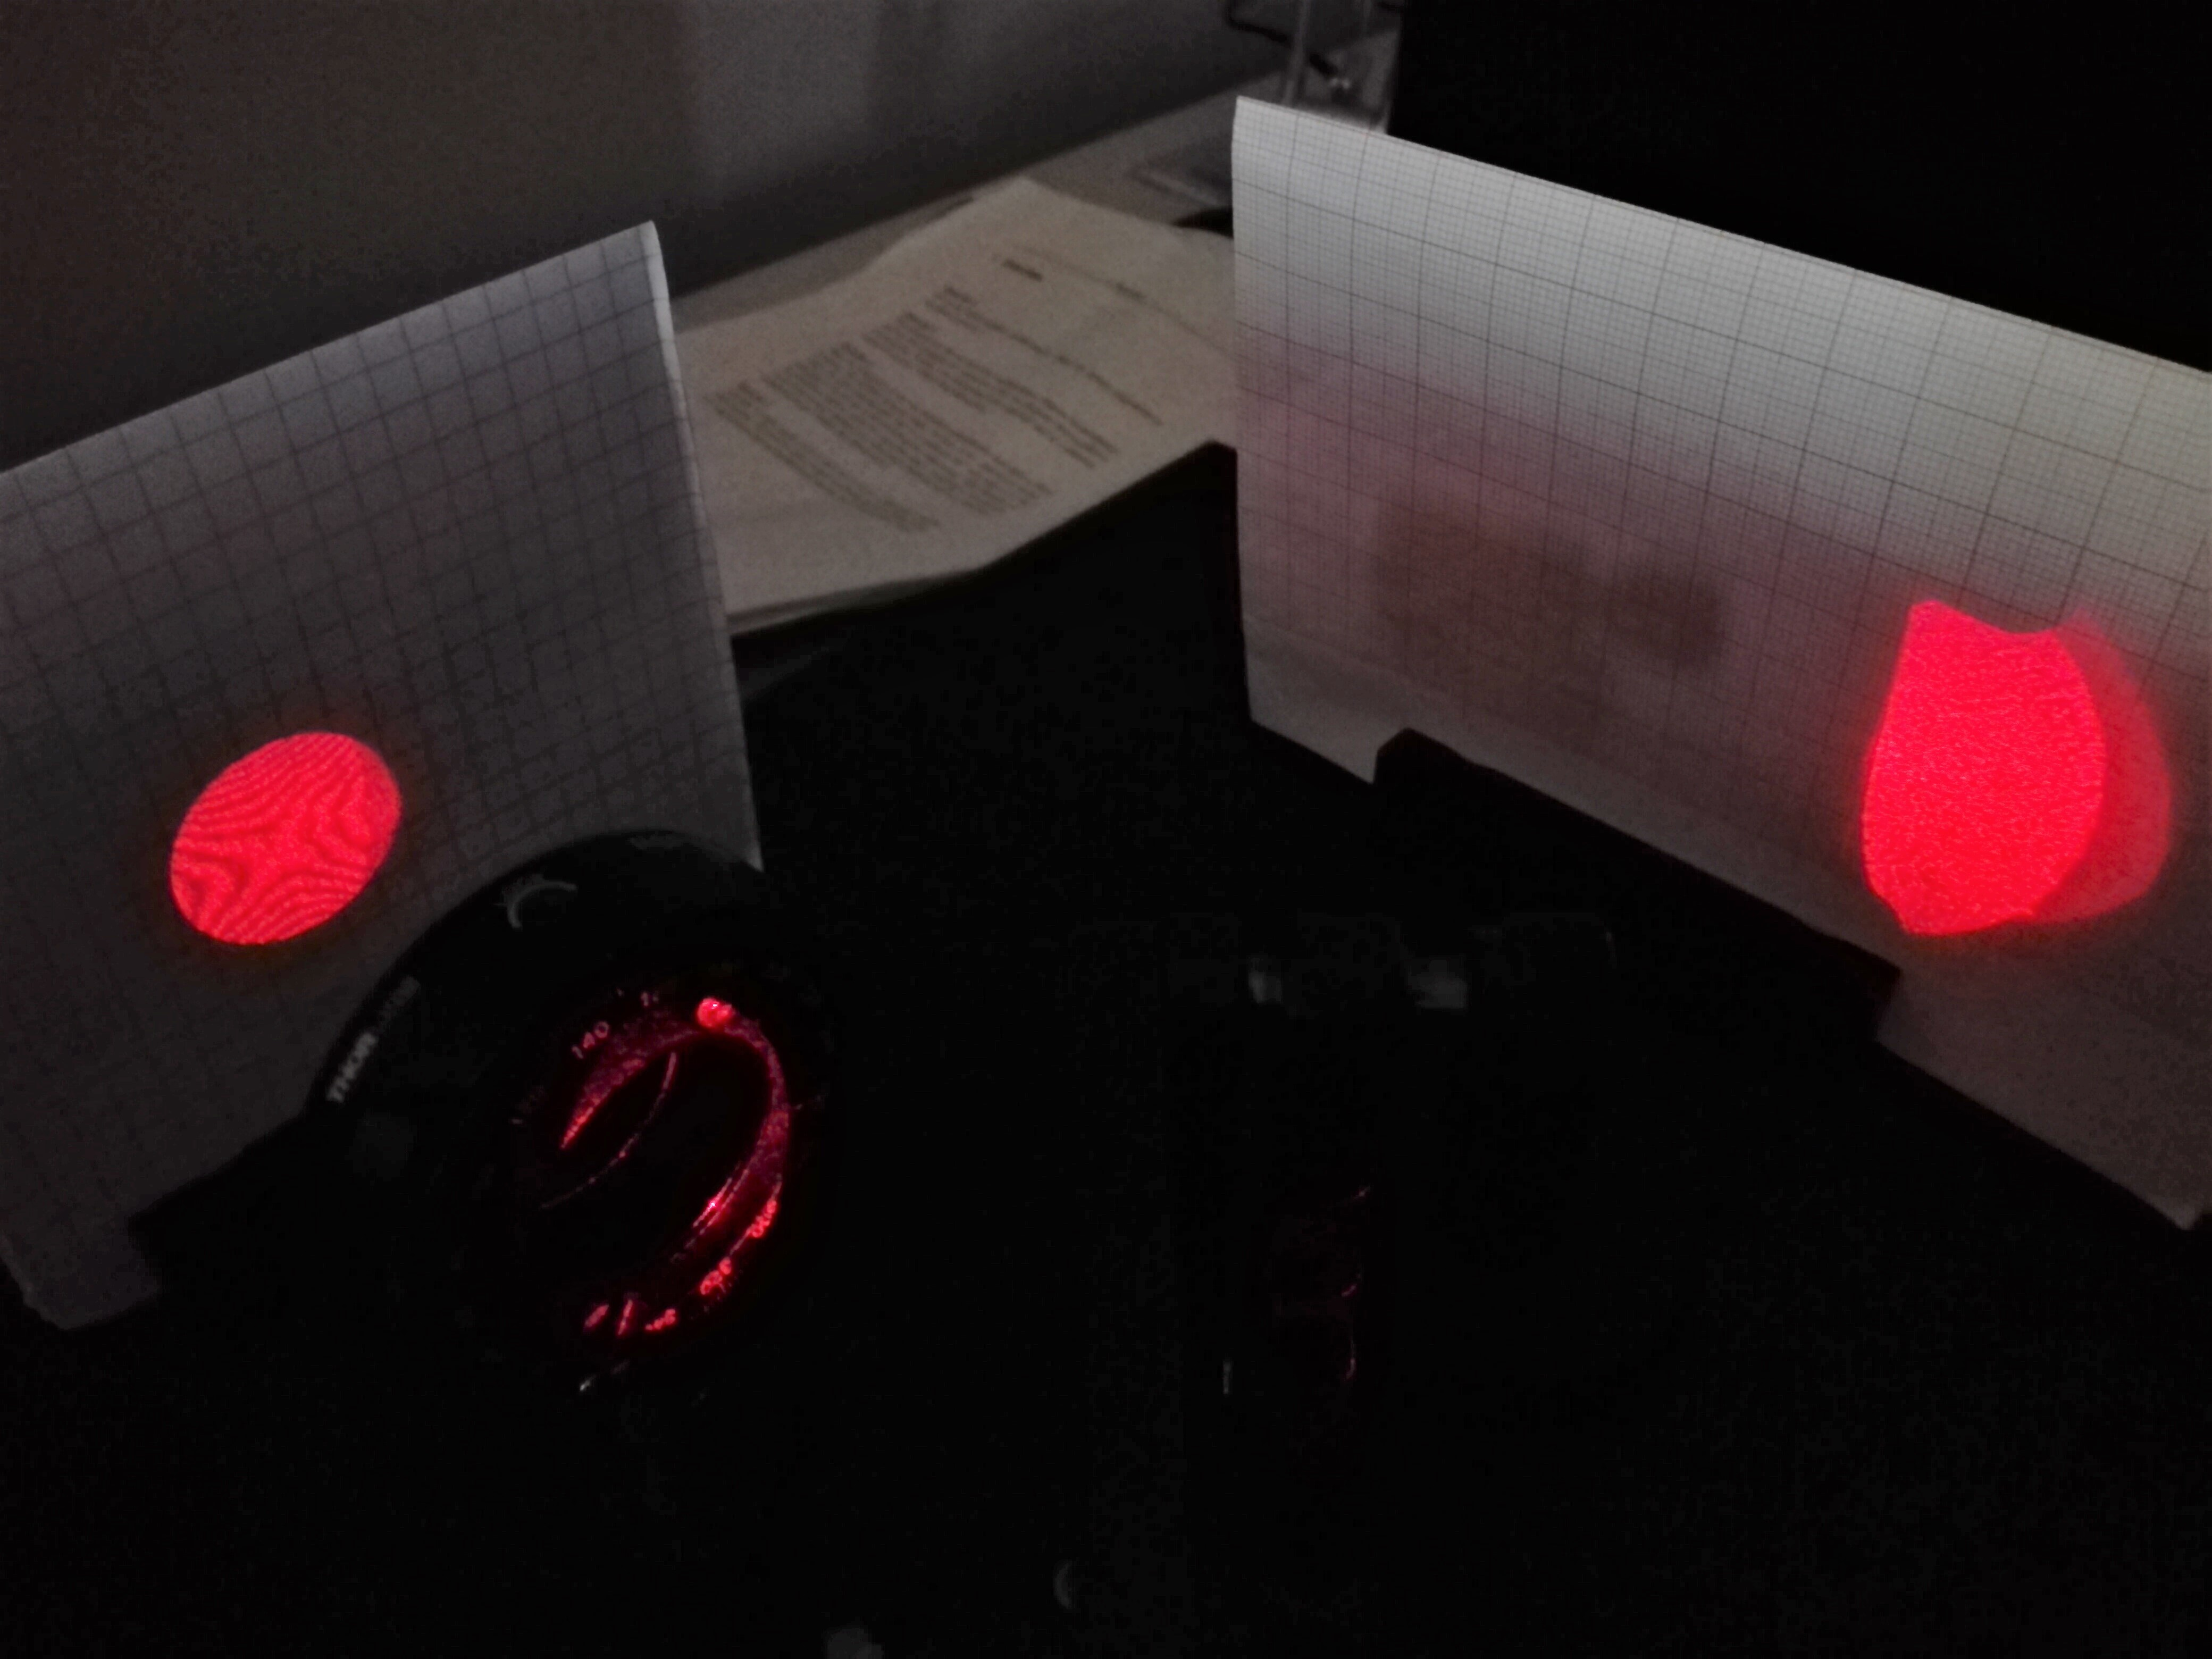
\includegraphics[scale=0.1]{images/radiert.jpg}
\caption{Aufnahme der beiden Auswertungsschirme bei Betrieb des Interferometers mit allen drei Polarisatoren. Auf dem rechten Schirm ist keine Interferenz zu erkennen, auf dem linken Schirm jedoch schon. Im Strahlengang des Musters des linken Schirms steht der Quantenradierer.}
\label{qrazge}
\end{figure}
Durch die Positionierung des Quantenradierers wird die Weg-Information der einfallenden Teilstrahlen gelöscht, da die resultierende Polarisation für beide Teilstrahlen gleich ist. Durch diesen Verlust der Weg-Information kann auf quantenmechanischer Ebene erneut Interferenz stattfinden.

\end{document}
